%%=========================================
\chapter{Introduction}
%This chapter gives an introduction to the use of \ac{czt} substrates to grow \ac{mct} films for \ac{ir} detectors. Then literature survey, problem formulation, and structure of the report.
% The first chapter of a well-structured thesis is always an introduction, setting the scene with background, problem description, objectives, limitations, and then looking ahead to summarise what is in the rest of the report. This is the part that readers look at first—so make sure it hooks them!

%\Ac{czt} is a substrate for epitaxial growth of lattice-matched \ac{mct} films used for infrared detectors. 

%Roughness, oxidation, defects, or contamination on the \ac{czt} surface can affect the growth of \ce{CdHgTe}. Hence, smooth and defect free surfaces are necessary to obtain high performance \ac{mct} infrared detectors.

%Chemo-mechanical polishing is used to obtain a smooth and planar surface. Both substrates are chemically etched in a bromine-methanol (\ce{Br-MeOH}) solution to remove the fine scratches that result from the chemo-mechanical polishing and the \ce{TeO2} layer that forms as the substrate is exposed to air.

The semiconducting material \ac{mct} is used to produce \acp{irfpa} for imaging of objects in the \ac{ir} region. The \ac{irfpa} consists of a 2-dimensional array of \ac{ir} detector elements at the focal plane of a lens. When an \ac{ir} photon with energy greater than the band gap is absorbed by the detector element, an electron will be excited from the valence band and placed in the conduction band. The charge, which is proportional to the number of absorbed photons, is collected at each detector element and converted to voltage by a \ac{roic} before the voltage signal is transferred to off-chip electronics. The measured signal from each detector element determine the intensity at the corresponding image pixel. The highest sensitivity \ac{mct} detector material is grown on lattice matched \ac{czt} substrates \citep{benson2016analysis}.
%An \ac{irfpa} operate by generating an electrical charge in relation to the number of photons that are detected at each pixel. 
%Electrical current, integrated decides the intensity of pixel. Pin hole/optics to make only photons from scenery if interest detected. 

%%=========================================
\section{Background}%\todo{Må skrive om denne seksjonen.}
% In this section, you should present the problem that you are going to investigate or analyze; why this problem is of interest; what has, so far, been done to solve the problem, and which parts of the problem that remain.

What makes the semiconducting material \ac{mct} suitable for \ac{ir} detectors, is the fact that it has high absorption, excellent lattice match with \ac{czt} substrates, and a tunable band gap which covers the entire \ac{ir} region from \SI{-0.26}{\electronvolt} to \SI{1.61}{\electronvolt} at \SI{77}{\kelvin} \citep{hansen1982energy}. Hence, the material can be adapted to detect \ac{ir} radiation in any of the \ac{ir} atmospheric transmission windows. The atmospheric transmission windows refer to the wavelength regions in which there is little absorption in the atmosphere: \ac{lwir} from \SI{8}{\micro\metre} to \SI{13}{\micro\metre}, \ac{mwir} from \SI{3}{\micro\metre} to \SI{5}{\micro\metre}, and \ac{swir} from \SI{1}{\micro\metre} to \SI{3}{\micro\metre}. An example of the atmospheric transmittance through 1 nautical mile, i.e. \SI{1.9}{\kilo\metre}, following a path at sea level can be seen in Fig.~\ref{fig:atm_window}. \Ac{ir} detection systems are usually designed to operate in these windows, so that radiation emitted from targets of interest can pass through the intermediate atmosphere and reach the detection system.
%to the transparent wavelength regions of the atmosphere. In the infrared region of the electromagnetic transmission spectra there can be seen an atmospheric window in the \ac{lwir}, that covers the wavelength range from \SI{8}{\micro\metre} to \SI{13}{\micro\metre}, and a fragmented atmospheric window can be observed in the \ac{swir} and \ac{mwir}, that covers the wavelength range from \SI{1}{\micro\metre} to \SI{3}{\micro\metre} and \SI{3}{\micro\metre} to \SI{5}{\micro\metre} respectively, see Fig.~\ref{fig:atm_window}.

\begin{figure}[htbp]
    \centering
    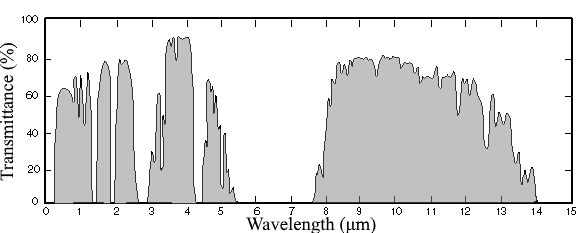
\includegraphics[width=0.8\columnwidth]{atmosfaerisk_spredning}
    \caption[Atmospheric transmittance versus wavelength.]{Atmospheric transmittance versus wavelength through 1 nautical mile (\SI{1.9}{\kilo\metre}) following a path at sea level. The transmittance is given in percent of total incoming radiation. A transmission window can be seen in the \acf{lwir} for wavelengths between \SI{8}{\micro\metre} and \SI{13}{\micro\metre} and a fragmented transmission window can be seen in the \acf{swir} and \acf{mwir} for wavelengths between \SI{0.2}{\micro\metre} and \SI{5}{\micro\metre}. The molecules mainly responsible for absorption are \ce{H2O}, \ce{CO2} and \ce{O2}. Modified from \citet{naval2013electronic}.}
    \label{fig:atm_window}
\end{figure}
%\mycomment{Indiker gjerne med piler, srkavering, sirkler eller på annen måte de vinsuene du har nevnt i teksten.}

The infrared detector applications of \ac{mct} and its consequential military role has made it a highly researched material, and it is used to make infrared detectors with high performance. In recent years, the technology has been increasingly utilised in many commercial products, e.g. medical diagnostics, drivers' enhanced vision, security applications and machine vision \citep{dhar2013advances}.
%Et materiale er vel ikke et forskningsfelt?  Materialet er interessant på grunn av egenskapene og de mulige anvendelsene, og det forskes på utvikling av ???  Framstillingsmetoder, materialegenskeper, anvendelser...?

\subsection{The Epitek Laboratory}

The Epitek laboratory at the \ac{ffi} is a laboratory for research on semiconducting materials. The main research focus is on growth of \ac{mct}, which is used in production of infrared detectors. This research consists of developing techniques and technologies for processing and characterising of both materials and components.

At the Epitek laboratory, \ac{czt} is used as a substrate material for both \ac{mbe} and \ac{lpe} growth of \ac{mct}. Epitaxy refers to the growth of a crystalline layer with a well-defined orientation determined by the crystal structure of the substrate. Defects, dislocations, impurities, and particles in and on the substrate will affect the growth and quality of the thin film layer. In the worst-case scenario, the processed \ac{ir} detector element will be defective due to the use of a poor \ac{mct} material. %in such a way that it becomes degraded, which in turn the processed \ac{ir} detector element defective.

The motivation for this study is the desire to obtain a better understanding of how impurities and defects on the \ac{czt} substrate surface affect the quality of the \ac{mct} films grown on the substrates. A long and tedious preparation process is required to get satisfying substrate surface quality for epitaxial growth \citep{triboulet2009cdteI}. Since the \ac{mct} detector material is grown directly on the \ac{czt} substrate, the as-received surface and the following pre-growth preparation of the surface are critical in the production of high quality detector material \citep{benson2015as-received}. It is important to grow films with high crystallinity, i.e. few grain boundaries and almost no dislocations, and few defects and impurities to ensure that the detector elements that are processed on the film function properly.

%%=========================================
\section{Literature Survey}%\todo{Må skrive om denne seksjonen.}
% You should here present the main books and articles that treat problems that are similar to what you are studying. If you, later in your thesis, describe the “state of the art” – with a detailed literature survey, you may just give a very brief survey here (approx. a quarter of a page). If this is the only literature survey, you need to go into more details. An objective of the literature survey is to show the reader that you are familiar with the main literature within your field of research – so that you do not “reinvent the wheel.”
%
% References to literature can be given in two different ways: 
% • As an explicit reference: It is shown by Lundteigen and Rausand (2008) and partly also by Rausand and Høyland (2004) that ...
% • As an implicit reference: It is shown (e.g., see Rausand and Høyland, 2004, Chap. 4) that ...
%
% In the example above, we have used “author-year” references, which is the preferred format.
%
% Remark: Following agreement with your supervisor, you may also refer by numbers, for example, [1]. 
%
% When you refer to the scientific literature, you should always write in present tense. Example: Rausand and Høyland (2004) show that ...
%
Defects in \ac{mbe}-grown \ac{mct} have been studied by many groups. \citet{selvig2007defects, selvig2008defects-a, selvig2008defects-b} at \ac{ffi} have described these defects as microvoids, hillocks, high temperature voids, needles, and dislocations. Microvoids are formed during growth at low substrate temperatures and can start at a defect or particle at the substrate surface. High temperature voids appear at higher temperatures, when \ce{Hg} evaporates from the film and leaves an excess of \ce{Te} which then collects in high temperature voids along with some polycrystalline \ce{CdTe} and \ac{mct}. The temperature where this occurs is called the tellurium phase limit.

A study of the impact of precipitates and contamination in \ac{czt} substrates on growth of \ac{mct} has been conducted by \citet{benson2014impact, benson2015as-received, benson2016analysis}. They studied state-of-the-art (211)B oriented \ac{czt} substrates for growth of \ac{mct} by \ac{mbe}. They associated two categories of \ac{mct} defects with defects originating in the substrate surface. The first was high temperature voids and bumps on the surface of \ac{mct} that were a result of tellurium precipitates in the underlying \ac{czt} substrate. The second was microvoid defects in the \ac{mct} film that originated in pits on the substrate surface. Their study of contamination on the as-received \ac{czt} substrates revealed polishing scratches,  residual polishing grit, \ce{Te} precipitates, \ce{Te} inclusions, \ac{czt} particles, and mounting wax. They observed that the residual polishing grit and mounting wax was removed by etching, but that the surface contamination of \ac{czt} particles was not removed by a standard \ac{mbe} preparation etch. %% substrates were from vendor A

%%=========================================
\section{Problem Formulation}%\todo{Må skrive om denne seksjonen.}
% You should define your problem in a clear an unambiguous way and explain why this is a problem, why it is of interest—and to whom. It is also important to delimit the problem area.
% OPPGAVEBESKRIVELSEN: Vi gror HgCdTe tynne filmer på \ac{czt} substrater. For å gro godt materiale, dvs med få defekter og dislokasjoner som kan degradere eller helt ødelegge et detektorelement, er det viktig at substratet har god krystallinitet, få defekter og få urenheter/partikler.   Oppgaven går ut på å karakterisere substratoverflaten etter forskjellig overflatebehandling og korrelere type/antall defekter i det grodde HgCdTe laget med substratpreparering og grobetingelser. Det vil bli bruk av flere av disse teknikkene: lysmikroskop, scanning electron microscope (SEM) med EDX, XPS, atomærkraftmikroskop (AFM), røntgen (XRD) og fotoluminesens (PL).
% Characterisation of substrate surfaces after different surface treatments and study the correlation between number of defects in the grown HgCdTe layer and preparation method and growth conditions. The following techniques will be used: optical microscopy, scanning electron microscope (SEM), atomic force microscopy (AFM), x-ray photoelectron spectroscopy (XPS) and photoluminescence (PL).
% Tittel: Comparative study of CdZnTe Substrates Prepared by Different Methods: Characterisation and properties
% Tittel: A study of CdZnTe Substrates Prepared by Different Methods: Characterisation and properties

This study was a continuation of the Specialisation Project in Physics where two as-received \ac{czt} substrates were characterised with optical microscopy, \ac{sem}, and \ac{eds}. In this study, a 3rd substrate was obtained and all three substrates were studied further. 

A characterisation of the surface of the substrates, both as-received and after surface pre-growth preparation, was performed. The substrates were first studied with optical microscopy to get an overview of the samples. To obtain higher resolution and more details, \ac{sem} with \ac{eds} was used to identify the different types of particles and features, as well as the composition of the substrate matrix. Near-\ac{ir} transmission microscopy was used to observe precipitates and inclusions throughout the substrate thickness. \Ac{afm} was used to get high resolution topographic mappings of the substrate surfaces, and \ac{ftir} was used to measure transmission spectra in a grid of points on the substrate. Finally, \iac{mct} film was grown on each substrate and the same characterisation was carried out to correlate the number of defects and type of defects in the grown \ac{mct} layer with the preparation of the substrate.

%while this study will examine one state-of-the-art (111)B-oriented \ac{czt} substrate from vendor A and one (111)B-oriented \ac{czt} substrate from vendor B for growth of \ac{mct} by \ac{lpe}, %\mycomment{Putte det etter , while ... et annet sted?}

%\todo{Få med dette et sted: It may well be the polishing that makes the substrates from vendor A the best on the market. Vendor A sells substrates to all the big detector companies in Europe and the US. Even though the substrates were not epi-ready as received, the surfaces were examined to observe what actually was present on the as-received surface followed by later studies of treatments to clean the surface. After the surface preparation was completed, the substrates were studied by \ac{sem} with \ac{eds}, optical microscopy, and \ac{afm}.}

%%=========================================
%\subsection{Objectives}
% The main objectives of this Master’s project are
% 1. This is the first objective
% 2. This is the second objective
% 3. This is the third objective
% 4. More objectives
%All objectives shall be stated such that we, after having read the thesis, can see whether or not you have met the objective. “To become familiar with . . . ” is therefore not a suitable objective. First of all, the objective of this project is to ... Having achived that, the next objectives are to ...

% MASTEROPPGAVE: Next, a characterisation of the substrates after different pre-growth preparations will be performed, and finally associate \ac{mct} film quality with substrate condition. 

%The objective of this project is to characterise the surface of as-received \ac{czt} substrates. This involves analysing the elemental composition of particles, scratches, defects, and impurities on the surface and the outermost atom layers. Having achieved a qualitative description of the surface of the substrates, the next objective is to get information about the concentration of defects and compare this for substrates from two different vendors.

%
%\subsection{What Remains to be Done?}
% After you have defined and delimited your problem – and presented the relevant results found in the literature within this field, you should sum up which parts of the problem that remain to be solved.
%%=========================================
%\section{Limitations}
% In this section you describe the limitations of your study. These may be related to the study object (physical limitations, operational limitations), to the thoroughness of the analysis, and so on.
%%=========================================
%\section{Approach}
% Here you should describe the (scientific) approach that you will use to solve the problem and meet your objectives. You should specify the approach for each objective. If there are any ethical problems related to your approach, these should be highlighted and discussed.
%%=========================================
\section{Structure of the Report}
% The introduction is composed of a problem formulation with objectives, motivation and approach.
The ordering of the text is as follows: Chapter~\ref{ch:methods} describes the characterisation methods that were used in the study. In Chapter~\ref{ch:exp-details}, the substrates, preparation methods, and experimental setup of the different characterisation methods are presented. Chapter~\ref{ch:results-and-discussion} presents the results and each result is discussed subsequently. Chapter~\ref{ch:conclusion} presents a summary and a conclusion. Lastly, recommendations for further work are proposed in Chapter~\ref{ch:further-work}.
%
%First the characterisation methods that were used in the study are described. Then, the substrates, preparation methods, and experimental setup of the different techniques are presented, followed by the corresponding results and discussion. Lastly, a conclusion and a description of further work are presented. %Then ... Lastly, a list of abbreviations and acronyms are presented in Appendix~\ref{app:acro}, and tables of photoelectron and Auger energies for the elements and compounds of interest are presented in Appendix~\ref{app:xps}.
% The rest of the report is structured as follows. Chapter 2 gives an introduction to . . .
% Remark: Notice that chapter and section headings shall be written in lowercase, but that all main words should start with a capital letter.
%%=========================================